\documentclass[border=0pt]{standalone}
\usepackage{amsmath}
\usepackage[usenames,dvipsnames]{xcolor}
\usepackage{graphicx}

%%font
\usepackage{euler}
\usepackage[OT1]{eulervm}
\renewcommand{\rmdefault}{pplx}

\usepackage{tikz}
\tikzset{roundnode/.style={circle,draw=black,fill=blue!20}}
\definecolor{TortugaColor}{rgb}{0.1,0.4,0.3}
\definecolor{Totemblue}{HTML}{09182F}
\definecolor{Totemred}{HTML}{2B030B}
\definecolor{Totemyellow}{HTML}{AD901B}
\usetikzlibrary{intersections}
%\usetikzlibrary{fadings}
\usetikzlibrary{arrows}
%\usetikzlibrary{arrows.meta}
%\usetikzlibrary{decorations}
\usetikzlibrary{decorations.pathmorphing}
\usetikzlibrary{decorations.text}
%\usetikzlibrary{fit}
%\usetikzlibrary{calc}
%\usetikzlibrary{through}
%\usetikzlibrary{positioning}
%\usetikzlibrary{graphs}
%\usetikzlibrary{mindmap}
%\usetikzlibrary{backgrounds}
%\usetikzlibrary{calligraphy}
\usepgfmodule{nonlineartransformations}
\usetikzlibrary{curvilinear}

%%% Set up polar step (code from the pgd manual)
%\makeatletter
%\def\polartransformation{%
% \pgf@x will contain the radius
% \pgf@y will contain the distance
%\pgfmathsincos@{\pgf@sys@tonumber\pgf@x}%
% pgfmathresultx is now the cosine of radius and
% pgfmathresulty is the sine of radius
%\pgf@x=\pgfmathresultx\pgf@y%
%\pgf@y=\pgfmathresulty\pgf@y%
%}
%\makeatother

\pgfdeclarelayer{background}
\pgfdeclarelayer{alpha}
\pgfdeclarelayer{beta}
\pgfsetlayers{background,alpha,main,beta}

%%pic TaiJi
\tikzset{
TaiJi/.pic={
\begin{scope}[thick,yi/.style={radius=0.4cm}]
\shade [draw=black] (0,0) circle [radius =3];
\shade [top color=black, bottom color=black!50,draw=black] (0,-3) arc [radius=3, start angle=-90, end angle=90]
arc [radius=1.5, start angle=90, end angle=270]
arc [radius=1.5, start angle=90, end angle=-90];
\draw[thin,fill=black] (0,-1.5) circle [yi];
\draw[thin,fill=white] (0,1.5) circle [yi];
\end{scope}
}}

%%pic Totu
\tikzset{
totu/.pic={
\begin{scope}[scale=0.2]
\pgfmathsetmacro{\legwidth}{0.4*0.2}
\draw[fill=green!60!black!30] (0,0.8) circle [x radius=0.3,y radius=0.4];
\foreach \i in {-1,1}{
\begin{scope}[xscale=\i]
\path (0.8,0) edge[draw=green!60!black!30,line width=\legwidth cm,line cap=round,bend left] ++(0.6,0);
\path (0.6,-1) edge[draw=green!60!black!30,line width=\legwidth cm,line cap=round] ++ (0.4,-0.4);
\end{scope}
}
\draw (0,-1.4) edge[draw=green!60!black!30,line width=\legwidth cm,line cap=round] ++ (0,-0.4);
\draw[fill=green!60!black,rounded corners] (1,0) -- (0,0.5) -- (-1,0) -- (-0.8,-1.2) -- (0,-1.6) -- (0.8,-1.2) -- cycle;
\end{scope}
}}

%%pic Rescuer
\tikzset{
Rescuer/.pic={
\begin{scope}[shift={(6.35,1.2)}]
\draw[fill=black!20!red!60!yellow] (-7,-0.8) -- (-6.7,-1.2) -- (-6,-1.2) -- (-5.7,-0.8) .. controls +(-0.3,-0.1) and +(0.3,-0.1) ..  cycle;
\end{scope}
}}

%%pic SatanHeart
\tikzset{
SatanHeart/.pic={
\pgfmathsetmacro{\SatanHradius}{1}
\pgfmathsetmacro{\LSatanHradius}{1.05}
\begin{scope}[very thick]
\draw[gray!80!blue, line width=2pt] (0,0) circle[radius=\LSatanHradius cm];
\draw[gray!80!blue] (-90:\SatanHradius) -- (-306:\SatanHradius) -- (-162:\SatanHradius) -- (-378:\SatanHradius) -- (-234:\SatanHradius) -- cycle;
\end{scope}
}}

%%pic Stone Gate
\tikzset{
stonegate/.pic={
\begin{scope}[gray]
\draw[fill,draw=none,rounded corners] (-1.3,-0.3) rectangle (-0.7,2);
\draw[fill,draw=none,rounded corners] (0.7,-0.3) rectangle (1.3,2);
\draw[fill,draw=none] (0,2) ellipse[x radius=2cm, y radius=0.3cm];
\end{scope}
}}
 
%%pic Ateles Zombia
\tikzset{
zombia/.pic={
\pgfmathsetmacro{\zombiascale}{0.2}
\begin{scope}[scale=\zombiascale]
\pgfmathsetmacro{\zombiawidth}{\zombiascale *0.3 cm}
\pgfmathsetmacro{\zombiabigcorner}{\zombiascale *4 pt}
\pgfmathsetmacro{\zombiasmallcorner}{\zombiascale *0.2 cm}
\begin{scope}[gray!40, rounded corners=\zombiabigcorner, line width=\zombiawidth, line cap=round]
%\node[circle,draw,thin] at (0,0) {};
\draw [fill,thin] (-1.9,0.4) circle [radius=0.3cm];
\draw (-1.8,0.1) -- (-2.2,-0.3) -- (-2.7,-0.6);
\draw (-1.8,0.1) -- (-1.6,-0.8) -- ++ (0.1,-0.1);
\draw (-1.8,0.1) -- (-0.9,0.1) -- (0.4,0.8);
\draw[rounded corners=\zombiasmallcorner] (0.4,0.8) -- ++ (0.3,0.2) -- ++ (0.2,-0.2);
\draw (0.7,1) -- (0.9,1.3) -- (1,2.5) -- (1.3,3) -- (1.8,2.9);
\draw (0.9,0.8) -- (0.9,0.5) -- (0.95,-0.3) -- (0.8,-1.1);
\draw (0.8,0.8) -- (0.4,0.6) -- (0,-0.7) -- ++(-0.2,-0.2);
\end{scope}
\end{scope}
}
}

%%pic family
\tikzset{
family/.pic={
\begin{scope}[xshift=-1cm]
\clip (0,0) rectangle (2,1);
\draw[fill] (0.25,0.7) circle [radius=0.1cm];
\draw[line cap=round,line width=0.06cm] (0.25,0.7) -- (0.25,0.2);
\draw[line cap=round,line width=0.06cm] (0.15,0) -- (0.25,0.2) -- (0.35,0);

\draw[fill] (0.75,0.6) circle [radius=0.1cm];
\draw[line cap=round,line width=0.06cm] (0.75,0.6) -- (0.75,0.2);
\draw[line cap=round,line width=0.06cm] (0.65,0) -- (0.75,0.2) -- (0.85,0);

\draw[fill] (1.25,0.6) circle [radius=0.1cm];
\draw[line cap=round,line width=0.06cm] (1.25,0.6) -- (1.25,0.2);
\draw[line cap=round,line width=0.06cm] (1.15,0) -- (1.25,0.2) -- (1.35,0);

\draw[fill] (1.75,0.65) circle [radius=0.1cm];
\draw[line cap=round,line width=0.06cm] (1.75,0.65) -- (1.75,0.2);
\draw[line cap=round,line width=0.06cm] (1.65,0) -- (1.75,0.2) -- (1.85,0);

\draw[line cap=round, line width=0.06cm] (0,0.3) -- (0.25,0.5) -- (0.5,0.3) -- (0.75,0.4) -- (1,0.3) -- (1.25,0.4) -- (1.5,0.3) -- (1.75,0.45) -- (2,0.3);
\end{scope}
}
}

\parindent=0pt

\begin{document}
%%2019NewYear
%% 16:9
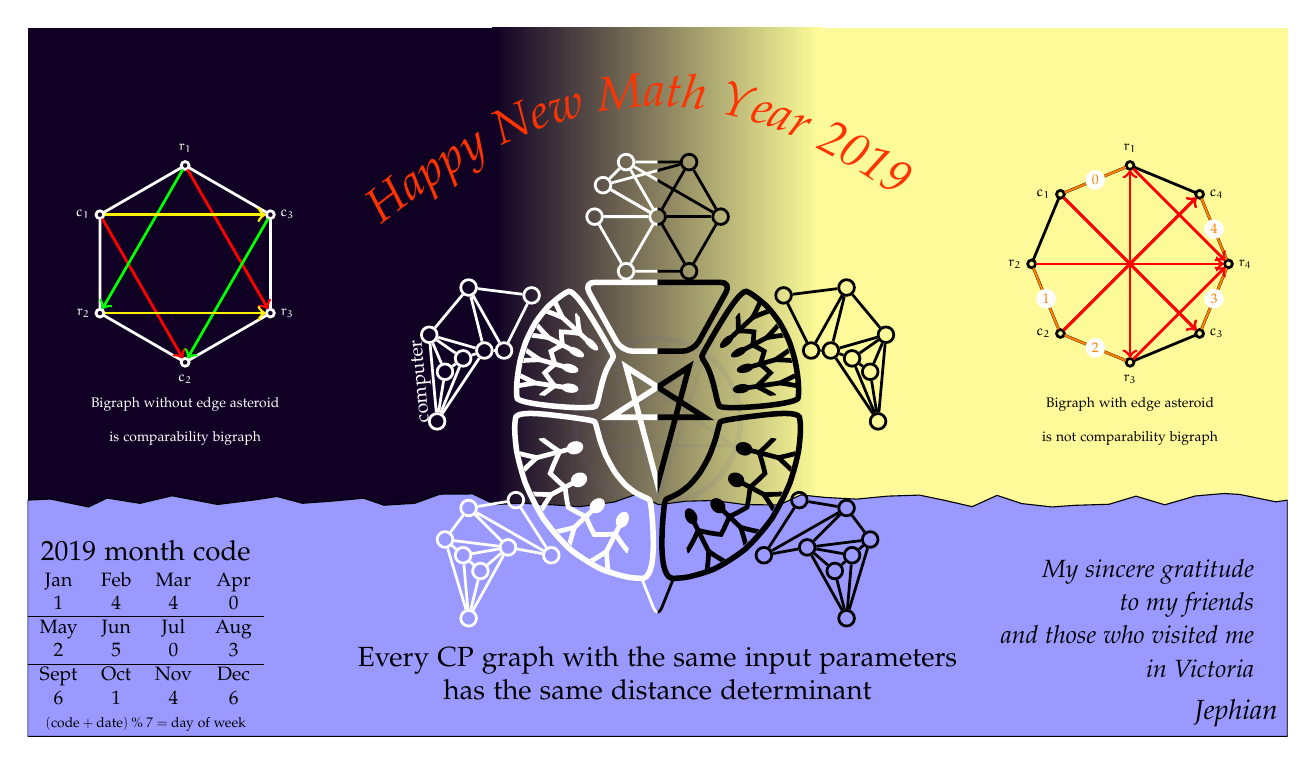
\begin{tikzpicture}
\coordinate (Jamaica) at (-8,-4);
\coordinate (Dominican) at (8,-4);
\coordinate (Cuba) at (-8,5);
\coordinate (TurksCaicos) at (8,5);
\coordinate (Tortuga) at (0,0);
\clip (Jamaica) rectangle (TurksCaicos);

%%Help Lines
\begin{pgfonlayer}{beta}
%\draw [step=1, black!50, thin] (Jamaica) grid (TurksCaicos);
%\draw (0,0) circle [radius=0.2cm];
\end{pgfonlayer}

%%background Layer
\begin{pgfonlayer}{background}
\fill[shade, draw=none, left color=red!30!blue!20!black, right color=yellow!40!white] (-2.1,-4) rectangle (2.1,5);
\fill[draw=none,red!30!blue!20!black] (Jamaica) rectangle (-2,5);
\fill[draw=none,yellow!40!white] (2,-4) rectangle (TurksCaicos);
%%SatanHeart
\pic[scale=1,opacity=0.1] at (0,0) {SatanHeart};
\end{pgfonlayer} 

%%Main Layer (main)
\begin{pgfonlayer}{main}
%%Tortuga
%\draw[fill=TortugaColor] decorate[decoration={name=random steps}] {(0,-1-|Dominican) ellipse [x radius=5cm, y radius=1.3cm]};
%%Sea
\draw[fill=blue!40,name path=sealevel] decorate[decoration={name=random steps}] {(0,-1 -| Jamaica) -- (0,-1 -| Dominican)} -- (Dominican) -- (Jamaica) -- cycle;

%%% Help lines for the turtle
%%% coordinates are also set here
\begin{scope}[opacity=0]
\foreach \i/\ang/\leng in {1/120/1,2/175/0.8,3/270/1,4/5/0.8,5/60/1}{
    \pgfmathsetmacro{\oleng}{\leng+1}
    \coordinate (to\i) at (\ang:\oleng);
    \coordinate (ti\i) at (\ang:\leng);
    \draw[red, very thick] (ti\i) -- (to\i);
}
\end{scope}

\foreach \r/\c in {1/white,-1/black}{
\begin{scope}[\c]
\pgfmathsetmacro{\leftend}{-2-2*\r}
\pgfmathsetmacro{\rightend}{2-2*\r}
\clip (\leftend,-3) rectangle (\rightend,5);
%%% Turtle head
\begin{scope}[every node/.style={circle, draw, inner sep=2pt}, yshift=2.6cm, scale=0.8, line width=1pt]
\node (1) at (0,0) {};
\foreach \v/\ang in {2/180,3/240,4/300,5/0,6/60,7/120,8/150}{
\node (\v) at (\ang:1) {};
\draw (1) -- (\v);
}
\draw (1) -- (2) -- (3) -- (4) -- (5) -- (6) -- (7) -- (8) -- (1);
\draw (5) -- (7);
\draw (6) -- (8);
\end{scope}
%%% Top turtle shell
\draw[rounded corners, line width=2pt] (118:2) -- (117:1) -- (63:1) -- (62:2) -- cycle;
%%% Center turtle shell
\draw[line width=2pt] (270:0.8) -- (60:0.8) -- (175:0.6) -- (5:0.6) -- (120:0.8) -- cycle;
%%% Turtle tail
\draw[line width=1pt, rounded corners] (-0.2,-2) -- (0,-2.5) -- (0.2,-2);
\end{scope}
}

%%% Upper turtle fins
\foreach \r/\c in {1/white,-1/black}{
\begin{scope}[every node/.style={circle, draw, inner sep=2pt},line width=1pt,xscale=\r, \c]
\node (1) at (-1.6,1.6) {};
\node (3) at (-2.4,1.7) {};
\node (5) at (-2.9,1.1) {};
\node (7) at (-2.8,0) {};
\node (2) at (-1.95,0.9) {};
\node (4) at (-2.2,0.9) {};
\node (6) at (-2.47,0.8) {};
\node (8) at (-2.7,0.63) {};
\draw (1) -- (3) -- (5) -- (7) -- (8) -- (6) -- (4) -- (2) -- (1);
\draw (2) -- (3) -- (4) -- (5) -- (6) -- (7);
\draw (4) -- (7);
\draw (5) -- (8);
\end{scope}
}

%%% Lower turtle fins
\foreach \r/\c in {1/white,-1/black}{
\begin{scope}[every node/.style={circle, draw, inner sep=2pt},line width=1pt,xscale=\r, \c]
\node (1) at (-1.8,-1) {};
\node (3) at (-2.4,-1.1) {};
\node (5) at (-2.7,-1.5) {};
\node (7) at (-2.4,-2.5) {};
\node (2) at (-1.35,-1.7) {};
\node (4) at (-1.9,-1.6) {};
\node (6) at (-2.47,-1.7) {};
\node (8) at (-2.25,-1.9) {};
\draw (1) -- (3) -- (5) -- (7) -- (8) -- (6) -- (4) -- (2) -- (1);
\draw (2) -- (3) -- (4) -- (5) -- (6) -- (7);
\draw (4) -- (7);
\draw (4) -- (8);
\end{scope}
}

%%% Upper left turtle shell
\begin{scope}[white]
\pgfsetcurvilinearbeziercurve
{\pgfpointpolar{120}{2cm}}
{\pgfpointadd{\pgfpointpolar{120}{2cm}}{\pgfpointpolar{210}{0.8cm}}}
{\pgfpointadd{\pgfpointpolar{175}{1.8cm}}{\pgfpointpolar{85}{0.5cm}}}
{\pgfpointpolar{175}{1.8cm}}
\makeatletter
\pgftransformnonlinear{\pgfpointcurvilinearbezierorthogonal\pgf@x\pgf@y}
\makeatother
\draw[line width=2pt] plot[smooth cycle,tension=0.2] coordinates{(0.15,0) (2.05,0) (2.05,1) (0.2,1)}--cycle;
\pic[xscale=0.85] at (1.1,0) {family};
\end{scope}

%%% Upper right turtle shell (this is quite unfortunate method to reflect the graph...)
\begin{scope}[black]
\pgfsetcurvilinearbeziercurve
{\pgfpointpolar{60}{2cm}}
{\pgfpointadd{\pgfpointpolar{60}{2cm}}{\pgfpointpolar{-30}{0.8cm}}}
{\pgfpointadd{\pgfpointpolar{5}{1.8cm}}{\pgfpointpolar{95}{0.5cm}}}
{\pgfpointpolar{5}{1.8cm}}
\makeatletter
\pgftransformnonlinear{\pgfpointcurvilinearbezierorthogonal\pgf@x\pgf@y}
\makeatother
\draw[line width=2pt] plot[smooth cycle,tension=0.2] coordinates{(0.15,0) (2.05,0) (2.05,-1) (0.2,-1)}--cycle;
\pic[xscale=-0.85,yscale=-1] at (1.1,0) {family};
\end{scope}

%%% Lower left turtle shell
\begin{scope}[white]
\pgfsetcurvilinearbeziercurve
{\pgfpointpolar{175}{1.8cm}}
{\pgfpointadd{\pgfpointpolar{175}{1.8cm}}{\pgfpointpolar{265}{0.8cm}}}
{\pgfpointadd{\pgfpointpolar{270}{2cm}}{\pgfpointpolar{180}{1.3cm}}}
{\pgfpointpolar{270}{2cm}}
\makeatletter
\pgftransformnonlinear{\pgfpointcurvilinearbezierorthogonal\pgf@x\pgf@y}
\makeatother
\draw[line width=2pt] plot[smooth cycle,tension=0.2] coordinates{(0.1,0) (2.4,0) (2.35,1) (0.2,1)}--cycle;
\pic[xscale=0.9] at (1.3,0) {family};
\end{scope}

%%% Lower right turtle shell (this is quite unfortunate method to reflect the graph...)
\begin{scope}[black]
\pgfsetcurvilinearbeziercurve
{\pgfpointpolar{5}{1.8cm}}
{\pgfpointadd{\pgfpointpolar{5}{1.8cm}}{\pgfpointpolar{-85}{0.8cm}}}
{\pgfpointadd{\pgfpointpolar{270}{2cm}}{\pgfpointpolar{0}{1.3cm}}}
{\pgfpointpolar{270}{2cm}}
\makeatletter
\pgftransformnonlinear{\pgfpointcurvilinearbezierorthogonal\pgf@x\pgf@y}
\makeatother
\draw[line width=2pt] plot[smooth cycle,tension=0.2] coordinates{(0.1,0) (2.4,0) (2.35,-1) (0.2,-1)}--cycle;
\pic[xscale=-0.9,yscale=-1] at (1.3,0) {family};
\end{scope}

\node[align=center] at (0,-3.2) {Every CP graph with the same input parameters\\ has the same distance determinant};

%%% Math and Computer 
\node[draw=none,opacity=0] at (0,0) {Mathematics};
\draw[decorate,decoration={raise=3pt, text along path, text={|\color{white}\scriptsize |computer}}] (-2.8,0) -- (-2.9,1.1);

%%% C8: with edge asteroid
\begin{scope}[every node/.style={circle, draw, inner sep=2pt, fill=none}, line width=1pt, shift={(6,2)}, scale=0.5, transform shape]
\node[label={above:$r_1$}] (r1) at (90:2.5) {};
\node[label={left:$r_2$}] (r2) at (180:2.5) {};
\node[label={below:$r_3$}] (r3) at (270:2.5) {};
\node[label={right:$r_4$}] (r4) at (0:2.5) {};
\node[label={left:$c_1$}] (c1) at (135:2.5) {};
\node[label={left:$c_2$}] (c2) at (225:2.5) {};
\node[label={right:$c_3$}] (c3) at (315:2.5) {};
\node[label={right:$c_4$}] (c4) at (45:2.5) {};
\draw (r1) -- (c1) -- (r2) -- (c2) -- (r3) -- (c3) -- (r4) -- (c4) -- (r1);

\draw[thick,orange] (r1) --node[midway,draw=none,fill=white] {0} (c1);
\draw[thick,orange] (r2) --node[midway,draw=none,fill=white] {1} (c2);
\draw[thick,orange] (c2) --node[midway,draw=none,fill=white] {2} (r3);
\draw[thick,orange] (c3) --node[midway,draw=none,fill=white] {3} (r4);
\draw[thick,orange] (r4) --node[midway,draw=none,fill=white] {4} (c4);

\foreach \x/\y in {r1/r3,c1/c3,r1/r4,c1/c3,r2/r4,c2/c4,r3/r4,c2/c4,r3/r1}{
\draw[red,->] (\x) -- (\y);
}
\end{scope}

\node[align=center] at (6,0) {\tiny Bigraph with edge asteroid\\ \tiny is not comparability bigraph}; 

%%% C6: without edge asteroid
\begin{scope}[white, every node/.style={circle, draw, inner sep=2pt, fill=none}, line width=1pt, shift={(-6,2)}, scale=0.5, transform shape]
\node[label={above:$r_1$}] (r1) at (90:2.5) {};
\node[label={left:$r_2$}] (r2) at (210:2.5) {};
\node[label={right:$r_3$}] (r3) at (330:2.5) {};
\node[label={left:$c_1$}] (c1) at (150:2.5) {};
\node[label={below:$c_2$}] (c2) at (270:2.5) {};
\node[label={right:$c_3$}] (c3) at (30:2.5) {};
\draw (r1) -- (c1) -- (r2) -- (c2) -- (r3) -- (c3) -- (r1);

\foreach \x/\y in {r1/r3,c1/c2}{
\draw[red,->] (\x) -- (\y);
}
\foreach \x/\y in {r1/r2,c3/c2}{
\draw[green,->] (\x) -- (\y);
}
\foreach \x/\y in {r2/r3,c1/c3}{
\draw[yellow,->] (\x) -- (\y);
}

\end{scope}

\node[align=center] at (-6,0) {\tiny\color{white} Bigraph without edge asteroid\\ \tiny\color{white} is comparability bigraph}; 

%%% gratitude
\node[yshift=1.5cm, xshift=-0.3cm, left,align=right] at (Dominican) {\it\small My sincere gratitude\\ \it\small to my friends\\ \it\small and those who visited me\\ \it\small in Victoria};


\end{pgfonlayer}


%%beta layer
\begin{pgfonlayer}{beta}

%%Happy New Math Year
\draw[decorate,decoration={text along path,text={|\color{red!80!yellow} \LARGE \it|Happy New Math Year 2019}}] (-3.5,2.5) .. controls (-1,4.5) and (1,4.5) .. (3.5,2.5);


%%Month code
\node[above] at (-6.5,-1.9) {2019 month code};
\node[scale=0.7,below] at (-6.5,-1.8) {\begin{tabular}{cccc} 
Jan & Feb & Mar & Apr \\
 1 & 4 & 4 & 0 \\
\hline
May & Jun & Jul & Aug \\
 2 & 5 & 0 & 3 \\
\hline
Sept & Oct & Nov & Dec \\
6 & 1 & 4 & 6 \\
\end{tabular}};
\node[scale=0.5,above] at (-6.5,-4) {$(\text{code}+\text{date})\mathbin{\%}7=\text{day of week}$};


%%Signature
\node[yshift=0.3cm,left] at (Dominican) {\it Jephian};

\end{pgfonlayer}




\end{tikzpicture}
\end{document}


%%\draw=\path[draw]
%%\clip=\path[clip]
%%\graph=\path[graph]
%%bend right ~ bend right=30 ~ in,out=right30, left 30
%%(left:2)=(180:2)
%%left ~ anchor=east ~ anchor 0
%%for sharp corners: line cap, line joint
%%for elliptical rectangle: smooth circle, plot coordinates, tensions
%For updating 2.10 to 3.0.0
%after moving the folder, it requires 
%sudo texhash 
% to make it work.
%%To convert to jpg: compile the pdf first, and then use the command below
%% convert -density 300 file.pdf -quality 90 file.jpg
%% required to install imagemagick

%% use pdf2png in AUR with Resolution 500 for 2018 
%% use gimp for 2019 (resolution 1890 x 1062, export quality 90)

%% Sample transformation as below
\makeatletter
\def\mytrans{
    \pgfmathparse{\pgf@x+1cm}
    %\pgf@x=\pgfmathresult pt
    \pgfmathsetlength{\pgf@x}{\pgfmathresult pt}
}
\makeatother


